\chapter{Algorismes greedy}

\index{algorisme greedy}

Un \key{algorisme greedy} (cobdiciós)
es aquell que construeix una solució al problema
fent sempre la tria que sembla
millor en aquell moment.
Un algorisme greedy mai desfà una opció
ja triada, sinó que construeix la solució
final directament.
Per aquest motiu, els algorismes greedy
solen ser molt eficients.

La dificultat de dissenyar algorismes greedy
és trobar una estratègia
que sempre produeixi una solució òptima
al problema.
En un algorisme greedy ha de passar que les eleccions
que són localment òptimes siguin també globalment òptimes.
Sovint no és fàcil d'argumentar perquè un algorisme greedy
concret funciona.

\section{Problema de les monedes}

Com a primer exemple, considerem un problema
on se'ns dóna un conjunt de monedes
i la nostra feina és formar una quantitat de diners $n$
fent servir les monedes.
Els valors de les monedes són
$\texttt{monedes}=\{c_1,c_2,\ldots,c_k\}$,
i cada moneda es pot utilitzar tantes vegades com vulguem.
Quin és el nombre mínim de monedes necessàries?

Per exemple, si les monedes són les monedes d'euro (en cèntims)
\[\{1,2,5,10,20,50,100,200\}\]
i $n=520$,
necessitem almenys quatre monedes.
La solució òptima és seleccionar monedes
$200+200+100+20$ la suma dels quals és 520.

\subsubsection{Algorisme greedy}

Un algorisme greedy senzill que resol el problema consisteix
en seleccionar sempre la moneda més gran possible,
fins que s'hagi construït la suma de diners requerida.
Aquest algorisme funciona en el cas d'exemple,
perquè primer seleccionem dues monedes de 200 cèntims,
després una moneda de 100 cèntims i finalment una moneda de 20 cèntims.
Però, com sabem que aquest algorisme sempre funciona?

Resulta que si les monedes són les monedes d'euro,
l'algorisme greedy \emph{sempre} funciona, és a dir,
sempre produeix una solució amb el mínim
nombre possible de monedes.
Això es pot argumentar de la manera següent:

En primer lloc, cada moneda 1, 5, 10, 50 i 100
pot aparèixer com a màxim una vegada en una solució òptima,
perquè si la solució contingués dues d'aquestes monedes,
podríem canviar-les per una sola moneda i
obtenir una solució millor.
Per exemple, si la solució contingués
les monedes $5+5$, podríem substituir-les per una moneda $10$.

De la mateixa manera, les monedes 2 i 20
només poden aparèixer com a màxim dues vegades en una
solució òptima, perquè d'altra forma podrem reemplaçar
les monedes $2+2+2$ per monedes $5+1$ i
les monedes $20+20+20$ per monedes $50+10$.
A més, una solució òptima no pot contenir
les monedes $2+2+1$ o $20+20+10$,
perquè podríem substituir-les per monedes $5$ i $50$.

Fent servir aquestes observacions,
hem de veure que per cada moneda $x$
no és possible construir de manera òptima
una suma $x$ o qualsevol suma més gran utilitzant només monedes
que són més petits que $x$.
Per exemple, si $x=100$, la suma òptima més gran fent
servir només monedes més petites és $50+20+20+5+2+2=99$.
Així, l'algorisme greedy que sempre selecciona
la moneda més gran produeix la solució òptima.

Aquest exemple mostra que pot ser difícil argumentar perquè un
algorisme greedy funciona, fins i tot si l'algorisme mateix és
simple.

\subsubsection{Cas general}

En el cas general, el conjunt de monedes pot contenir qualsevol moneda
i l'algorisme greedy ja \emph{no} produeix necessàriament
una solució òptima.

Podem demostrar que un algorisme greedy no funciona
mostrant un contraexemple
on l'algorisme ens dóna una resposta incorrecta.
En aquest problema és fàcil trobar-ne un:
si les monedes són $\{1,3,4\}$ i la suma objectiu
és 6, l'algorisme greedy produeix la solució
$4+1+1$ mentre que la solució òptima és $3+3$.

No se sap si el problema generalitzat de la moneda
es pot resoldre fent servir algun algorisme greedy\footnote{
No obstant això, és possible
\emph{comprovar} en temps polinòmic
si l'algorisme greedy que s'ha presentat en aquest capítol funciona
amb un conjunt determinat de monedes \cite{pea05}.}.
Tanmateix, com veurem al capítol 7,
en alguns casos el problema generalitzat pot ser
resolt eficientment fent servir un algorisme de programació
dinàmica que sempre dóna la resposta correcta.

\section{Scheduling}

Molts problemes de \emph{scheduling} (planificació horària)
es poden resoldre fent servir algorismes greedy.
Un problema clàssic és el següent:
donats $n$ esdeveniments amb els corresponents temps d'inici i
de final, troba un scheduling
que inclogui tants esdeveniments com sigui possible.
No és permet seleccionar un esdeveniment parcialment.
Per exemple, considerem els esdeveniments següents:
\begin{center}
\begin{tabular}{lll}
esdeveniment & hora d'inici & hora final \\
\hline
$A$ & 1 & 3 \\
$B$ & 2 & 5 \\
$C$ & 3 & 9 \\
$D$ & 6 & 8 \\
\end{tabular}
\end{center}
En aquest cas, el nombre màxim d'esdeveniments és dos.
Per exemple, podem seleccionar els esdeveniments $B$ i $D$
com segueix:
\begin{center}
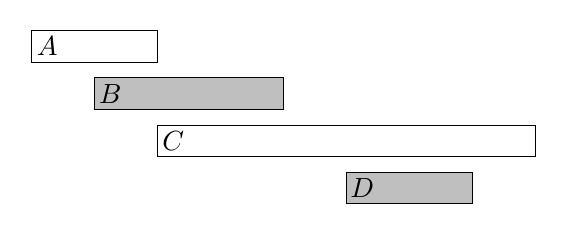
\begin{tikzpicture}[scale=.4]
  \begin{scope}
    \draw (2, 0) rectangle (6, -1);
    \draw[fill=lightgray] (4, -1.5) rectangle (10, -2.5);
    \draw (6, -3) rectangle (18, -4);
    \draw[fill=lightgray] (12, -4.5) rectangle (16, -5.5);
    \node at (2.5,-0.5) {$A$};
    \node at (4.5,-2) {$B$};
    \node at (6.5,-3.5) {$C$};
    \node at (12.5,-5) {$D$};
  \end{scope}
\end{tikzpicture}
\end{center}

És possible inventar diversos algorismes greedy
per al problema, però quin d'ells funciona en tots els casos?

\subsubsection*{Algorisme 1}

La primera idea és començar seleccionant els
esdeveniments més \emph{curts} possibles.
En l'exemple anterior l'algorisme selecciona els següent
esdeveniments:
\begin{center}
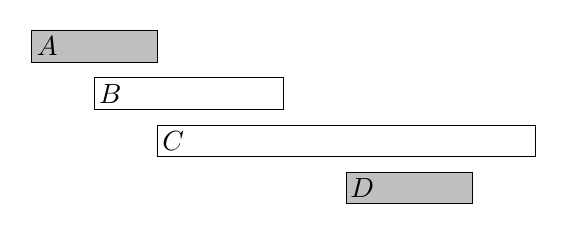
\begin{tikzpicture}[scale=.4]
  \begin{scope}
    \draw[fill=lightgray] (2, 0) rectangle (6, -1);
    \draw (4, -1.5) rectangle (10, -2.5);
    \draw (6, -3) rectangle (18, -4);
    \draw[fill=lightgray] (12, -4.5) rectangle (16, -5.5);
    \node at (2.5,-0.5) {$A$};
    \node at (4.5,-2) {$B$};
    \node at (6.5,-3.5) {$C$};
    \node at (12.5,-5) {$D$};
  \end{scope}
\end{tikzpicture}
\end{center}

Tanmateix, seleccionar esdeveniments curts no sempre és
una estratègia correcta. Per exemple, l'algorisme falla
en el cas següent:
\begin{center}
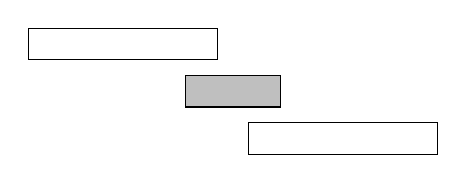
\begin{tikzpicture}[scale=.4]
  \begin{scope}
    \draw (1, 0) rectangle (7, -1);
    \draw[fill=lightgray] (6, -1.5) rectangle (9, -2.5);
    \draw (8, -3) rectangle (14, -4);
  \end{scope}
\end{tikzpicture}
\end{center}
Si seleccionem l'esdeveniment més curt, només podem seleccionar
un, quan en realitat seria possible seleccionar-ne dos.

\subsubsection*{Algorisme 2}

Una altra idea és seleccionar sempre l'esdeveniment
que \emph{comença} tan d'hora com sigui possible.
Aquest algorisme selecciona els esdeveniments següents:
\begin{center}
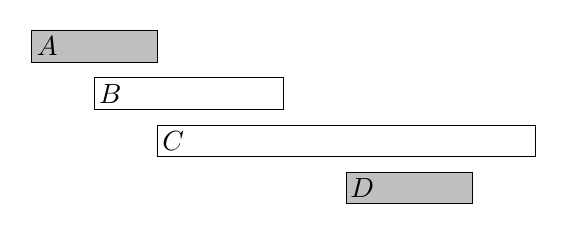
\begin{tikzpicture}[scale=.4]
  \begin{scope}
    \draw[fill=lightgray] (2, 0) rectangle (6, -1);
    \draw (4, -1.5) rectangle (10, -2.5);
    \draw (6, -3) rectangle (18, -4);
    \draw[fill=lightgray] (12, -4.5) rectangle (16, -5.5);
    \node at (2.5,-0.5) {$A$};
    \node at (4.5,-2) {$B$};
    \node at (6.5,-3.5) {$C$};
    \node at (12.5,-5) {$D$};
  \end{scope}
\end{tikzpicture}
\end{center}

Tanmateix, també podem trobar un contraexemple
per a aquest algorisme.
Per exemple, en el cas següent,
l'algorisme només selecciona un esdeveniment:
\begin{center}
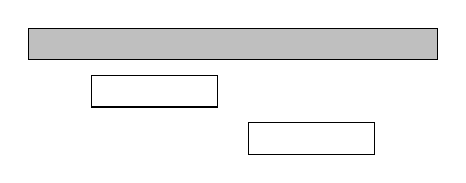
\begin{tikzpicture}[scale=.4]
  \begin{scope}
    \draw[fill=lightgray] (1, 0) rectangle (14, -1);
    \draw (3, -1.5) rectangle (7, -2.5);
    \draw (8, -3) rectangle (12, -4);
  \end{scope}
\end{tikzpicture}
\end{center}
Si seleccionem el primer esdeveniment, ja no és possible
seleccionar-ne cap d'altre, quan en realitat hauríem pogut
seleccionar dos esdeveniments

\subsubsection*{Algorisme 3}

La tercera idea és seleccionar l'esdeveniment que
\emph{acabi} tan \emph{d'hora} com sigui possible.
Aquest algorisme selecciona els esdeveniments següents:
\begin{center}
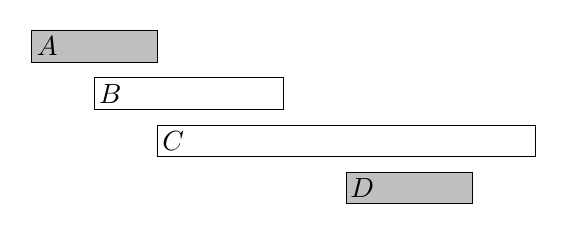
\begin{tikzpicture}[scale=.4]
  \begin{scope}
    \draw[fill=lightgray] (2, 0) rectangle (6, -1);
    \draw (4, -1.5) rectangle (10, -2.5);
    \draw (6, -3) rectangle (18, -4);
    \draw[fill=lightgray] (12, -4.5) rectangle (16, -5.5);
    \node at (2.5,-0.5) {$A$};
    \node at (4.5,-2) {$B$};
    \node at (6.5,-3.5) {$C$};
    \node at (12.5,-5) {$D$};
  \end{scope}
\end{tikzpicture}
\end{center}

Resulta que aquest algorisme
\emph{sempre} produeix una solució òptima.

Perquè l'algorisme funciona?  Sigui $X$ l'esdeveniment que acaba
primer, i considerem una solució òptima que no tingui $X$. Com
que $X$ és l'esdeveniment que acaba primer, podem intercanviar
el primer element de la solució òptima per $X$ sense
causar cap conflicte. Per tant, per a qualsevol solució òptima
sense $X$, n'existeix una altra solució òptima amb $X$. Això demostra
que la primera tria de l'algorisme no és errònia. El mateix argument
s'aplica a les següents tries.

\section{Tasques i terminis}

Considerem ara un problema on
se'ns dóna $n$ tasques amb durades i terminis
i la nostra feina és triar en quin ordre s'han de fer les tasques.
Per a cada tasca, guanyem $d-x$ punts
on $d$ és la data límit de la tasca
i $x$ és el moment en què acabem la tasca.
Quina és la puntuació total més gran
que podem obtenir?

Per exemple, suposem que les tasques són les següents:
\begin{center}
\begin{tabular}{lll}
tasca & durada & termini \\
\hline
$A$ & 4 & 2 \\
$B$ & 3 & 5 \\
$C$ & 2 & 7 \\
$D$ & 4 & 5 \\
\end{tabular}
\end{center}
En aquest cas, aquesta és una assignació òptima:
\begin{center}
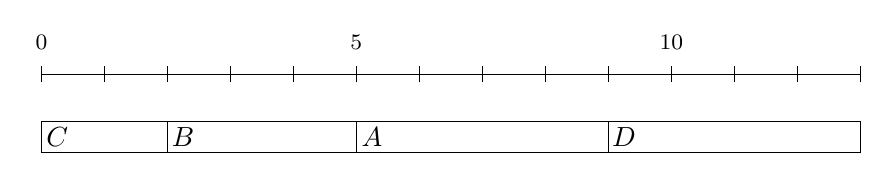
\begin{tikzpicture}[scale=.4]
  \begin{scope}
    \draw (0, 0) rectangle (4, -1);
    \draw (4, 0) rectangle (10, -1);
    \draw (10, 0) rectangle (18, -1);
    \draw (18, 0) rectangle (26, -1);
    \node at (0.5,-0.5) {$C$};
    \node at (4.5,-0.5) {$B$};
    \node at (10.5,-0.5) {$A$};
    \node at (18.5,-0.5) {$D$};

    \draw (0,1.5) -- (26,1.5);
    \foreach \i in {0,2,...,26}
    {
        \draw (\i,1.25) -- (\i,1.75);
    }
    \footnotesize
    \node at (0,2.5) {0};
    \node at (10,2.5) {5};
    \node at (20,2.5) {10};

  \end{scope}
\end{tikzpicture}
\end{center}
En aquesta solució, $C$ ens dóna 5 punts,
$B$ ens dóna 0 punts, $A$ ens dóna -7$ punts
i $D$ ens dóna -8$ punts,
per tant, la puntuació total és de $-10$.

Sorprenentment, la solució òptima a aquest problema
no depèn en absolut dels terminis.
Una estratègia greedy correcta és simplement
realitzar les tasques \emph{ordenades per la seva durada}
en ordre creixent.
La raó d'això és que si mai fem
dues tasques una darrere l'altra de manera que la primera tasca
triga més que la segona tasca, podem millorar la solució
intercanviant les tasques. Per exemple, considerem
l'assignació següent:
\begin{center}
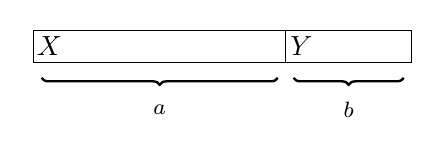
\begin{tikzpicture}[scale=.4]
  \begin{scope}
    \draw (0, 0) rectangle (8, -1);
    \draw (8, 0) rectangle (12, -1);
    \node at (0.5,-0.5) {$X$};
    \node at (8.5,-0.5) {$Y$};

\draw [decoration={brace}, decorate, line width=0.3mm] (7.75,-1.5) -- (0.25,-1.5);
\draw [decoration={brace}, decorate, line width=0.3mm] (11.75,-1.5) -- (8.25,-1.5);

\footnotesize
\node at (4,-2.5) {$a$};
\node at (10,-2.5) {$b$};

  \end{scope}
\end{tikzpicture}
\end{center}
Com que es dóna $a>b$, hauríem d'intercanviar les tasques:
\begin{center}
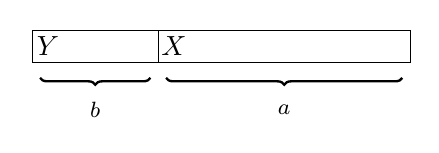
\begin{tikzpicture}[scale=.4]
  \begin{scope}
    \draw (0, 0) rectangle (4, -1);
    \draw (4, 0) rectangle (12, -1);
    \node at (0.5,-0.5) {$Y$};
    \node at (4.5,-0.5) {$X$};

\draw [decoration={brace}, decorate, line width=0.3mm] (3.75,-1.5) -- (0.25,-1.5);
\draw [decoration={brace}, decorate, line width=0.3mm] (11.75,-1.5) -- (4.25,-1.5);

\footnotesize
\node at (2,-2.5) {$b$};
\node at (8,-2.5) {$a$};

  \end{scope}
\end{tikzpicture}
\end{center}
Ara $X$ ens dóna $b$ punts menys però $Y$ ens dóna $a$ punts més,
de manera que la puntuació total augmenta en $a-b > 0$.
En una solució òptima,
per cada dues tasques consecutives qualsevol,
la tasca més curta s'ha de fer abans que la tasca més llarga.
Per tant, les tasques s'han de fer ordenades
en funció de la seva durada.

\section{Minimitzar sumes}

Considerem el problema on
se'ns donen $n$ nombres $a_1,a_2,\ldots,a_n$
i la nostra tasca és trobar un valor $x$
que minimitzi la suma
\[|a_1-x|^c+|a_2-x|^c+\cdots+|a_n-x|^c.\]
Ens centrem en els casos $c=1$ i $c=2$.

\subsubsection{Cas $c=1$}

En aquest cas hem de minimitzar la suma
\[|a_1-x|+|a_2-x|+\cdots+|a_n-x|.\]
Per exemple, si els números són $[1,2,9,2,6]$,
la millor solució és seleccionar $x=2$
que produeix la suma
\[
|1-2|+|2-2|+|9-2|+|2-2|+|6-2|=12.
\]
En el cas general, la millor opció per $x$
és la \textit{mediana} dels nombres,
és a dir, el nombre del mig després d'ordenar-los.
Per exemple, la llista $[1,2,9,2,6]$
es converteix en $[1,2,2,6,9]$ després d'ordenar,
i la mediana és 2.

La mediana és una opció òptima,
perquè si $x$ és més petit que la mediana,
la suma es fa més petita en augmentar $x$,
i si $x$ és més gran que la mediana,
la suma es fa més petita en disminuir $x$.
Per tant, la solució òptima és que $x$
sigui la mediana.
Si $n$ és parell i hi ha dues medianes,
qualsevol de les medianes o els valors entre les dues
són òptimes.

\subsubsection{Cas $c=2$}

En aquest cas, hem de minimitzar la suma
\[(a_1-x)^2+(a_2-x)^2+\cdots+(a_n-x)^2.\]
Per exemple, si els nombres són $[1,2,9,2,6]$,
la millor solució és seleccionar $x=4$
que dóna lloc a la suma
\[
(1-4)^2+(2-4)^2+(9-4)^2+(2-4)^2+(6-4)^2=46.
\]
En el cas general, la millor opció per $x$
és la \emph{mitjana} dels nombres.
A l'exemple, la mitjana és $(1+2+9+2+6)/5=4$.
Aquest resultat s'obté presentant
la suma de la següent manera:
\[
nx^2 - 2x(a_1+a_2+\cdots+a_n) + (a_1^2+a_2^2+\cdots+a_n^2)
\]
Podem ignorar l'última part perquè no depèn de $x$.
Les parts restants formen una funció
$nx^2-2xs$ on $s=a_1+a_2+\cdots+a_n$.
Aquesta és una paràbola que s'obre cap amunt
amb arrels $x=0$ i $x=2s/n$. El valor mínim
és la mitjana de les arrels $x=s/n$, és a dir,
la mitjana dels nombres $a_1,a_2,\ldots,a_n$.

\section{Compressió de dades}

\index{compressió de dades}
\index{codificació binària}
\index{codi}

Una \key{codificació binària} assigna a cada caràcter
d'una cadena un \key{codi} format per bits.
Podem \emph{comprimir} la cadena fent servir la codificació
que reemplaça cada caràcter pel
seu codi corresponent.
Per exemple, la següent codificació assigna aquests
codis als caràcters:
\texttt{A}–\texttt{D}:
\begin{center}
\begin{tabular}{rr}
caràcter & codi \\
\hline
\texttt{A} & 00 \\
\texttt{B} & 01 \\
\texttt{C} & 10 \\
\texttt{D} & 11 \\
\end{tabular}
\end{center}
Aquesta codificació té \key{longitud constant}
perquè cada codi té la mateixa mida.
Fent servir aquesta codificació, la cadena
\texttt{AABACDACA} es transforma en els 18 bits 
\[00\,00\,01\,00\,10\,11\,00\,10\,00\].
Tanmateix, podem comprimir encara més la cadena
si fem servir codificacions de \key{longitud variable}, on
cada codi pot tenir longituds diferents.
D'aquesta manera podem fer servir codis curts pels caràcters que
apareixen sovint i codis llargs pels caràcters infreqüents.
Resulta que la següent codificació és \key{òptima}
per a la cadena anterior:
\begin{center}
\begin{tabular}{rr}
caràcter & codi \\
\hline
\texttt{A} & 0 \\
\texttt{B} & 110 \\
\texttt{C} & 10 \\
\texttt{D} & 111 \\
\end{tabular}
\end{center}
Una codificació òptima comprimeix la cadena en el mínim
espai possible.
En aquest cas, la cadena comprimida
\[0\,0\,110\,0\,10\,111\,0\,10\,0,\]
només necessita 15 bits en lloc de 18. Fer servir la millor
codifcació ens estalvia 3 bits.

Exigim també que no hi hagi cap codi que sigui
prefix d'un altre codi.
Per exemple, està prohibit que la codificació
contingui els codis $10$ i $1011$.
El motiu es que volem
poder recuperar la cadena original
a partir de la cadena comprimida.
Si un codi pogués ser prefix d'un altre
això no sempre seria possible.
Per exemple, la codificació següent \emph{no} és vàlida:
\begin{center}
\begin{tabular}{rr}
caràcter & codi \\
\hline
\texttt{A} & 10 \\
\texttt{B} & 11 \\
\texttt{C} & 1011 \\
\texttt{D} & 111 \\
\end{tabular}
\end{center}
Amb aquesta codificació, no sabem si $1011$ és la compressió
de \texttt{AB} o de \texttt{C}.

\index{Codificació de Huffman}

\subsubsection{Codificació de Huffman}

La \key{codificació de Huffman}\footnote{D. A. Huffman va descobrir
aquest mètode en un treball de final de curs a l'universitat
i va publicar l'algorisme el 1952 \cite{huf52}.} és un algorisme
greedy que construeix una codificació òptima per
a comprimir una cadena determinada.
L'algorisme construeix un arbre binari
en funció de les freqüències dels caràcters
de la cadena,
i trobem el codi que assignem a cada caràcter
recorrent un camí des de l'arrel fins al node
corresponent.
Quan cop que ens movem a l'esquerra escrivim un bit 0,
i quan ens movem a la dreta escrivim un bit 1.

Inicialment, cada caràcter és un node el pes del qual és el
nombre de vegades que el caràcter apareix a la cadena.
A continuació, combinem els dos nodes de pes mínim
per a crear un nou node el pes del qual és la suma dels
pesos dels nodes originals.
El procés continua fins que combinem tots els nodes.

A continuació mostrem com es crea el codi de Huffman
per a la cadena \texttt{AABACDACA}.
Al principi, hi ha quatre nodes, un per cada caràcter
de la cadena:

\begin{center}
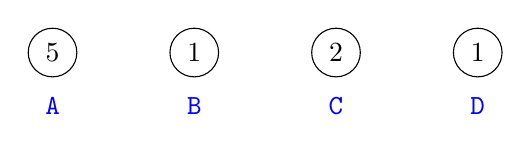
\begin{tikzpicture}[scale=0.9]
\node[draw, circle] (1) at (0,0) {$5$};
\node[draw, circle] (2) at (2,0) {$1$};
\node[draw, circle] (3) at (4,0) {$2$};
\node[draw, circle] (4) at (6,0) {$1$};

\node[color=blue] at (0,-0.75) {\texttt{A}};
\node[color=blue] at (2,-0.75) {\texttt{B}};
\node[color=blue] at (4,-0.75) {\texttt{C}};
\node[color=blue] at (6,-0.75) {\texttt{D}};

%\path[draw,thick,-] (4) -- (5);
\end{tikzpicture}
\end{center}
El node que representa el caràcter \texttt{A}
té pes 5 perquè el caràcter \texttt{A}
apareix 5 vegades a la cadena, i el mateix per la
resta de pesos.

El primer pas és combinar els nodes dels
caràcters \texttt{B} i \texttt{D}, tots dos amb pes 1.
El resultat és:
\begin{center}
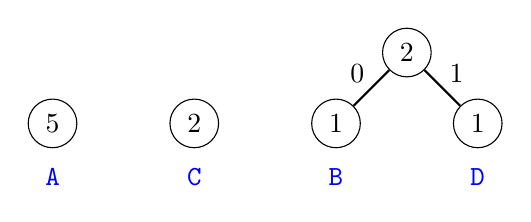
\begin{tikzpicture}[scale=0.9]
\node[draw, circle] (1) at (0,0) {$5$};
\node[draw, circle] (3) at (2,0) {$2$};
\node[draw, circle] (2) at (4,0) {$1$};
\node[draw, circle] (4) at (6,0) {$1$};
\node[draw, circle] (5) at (5,1) {$2$};

\node[color=blue] at (0,-0.75) {\texttt{A}};
\node[color=blue] at (2,-0.75) {\texttt{C}};
\node[color=blue] at (4,-0.75) {\texttt{B}};
\node[color=blue] at (6,-0.75) {\texttt{D}};

\node at (4.3,0.7) {0};
\node at (5.7,0.7) {1};

\path[draw,thick,-] (2) -- (5);
\path[draw,thick,-] (4) -- (5);
\end{tikzpicture}
\end{center}
Després d'això, combinen els nodes amb pes 2:
\begin{center}
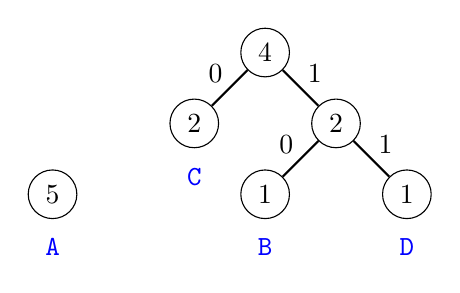
\begin{tikzpicture}[scale=0.9]
\node[draw, circle] (1) at (1,0) {$5$};
\node[draw, circle] (3) at (3,1) {$2$};
\node[draw, circle] (2) at (4,0) {$1$};
\node[draw, circle] (4) at (6,0) {$1$};
\node[draw, circle] (5) at (5,1) {$2$};
\node[draw, circle] (6) at (4,2) {$4$};

\node[color=blue] at (1,-0.75) {\texttt{A}};
\node[color=blue] at (3,1-0.75) {\texttt{C}};
\node[color=blue] at (4,-0.75) {\texttt{B}};
\node[color=blue] at (6,-0.75) {\texttt{D}};

\node at (4.3,0.7) {0};
\node at (5.7,0.7) {1};
\node at (3.3,1.7) {0};
\node at (4.7,1.7) {1};

\path[draw,thick,-] (2) -- (5);
\path[draw,thick,-] (4) -- (5);
\path[draw,thick,-] (3) -- (6);
\path[draw,thick,-] (5) -- (6);
\end{tikzpicture}
\end{center}
Finalment, combinen els dos nodes restants:
\begin{center}
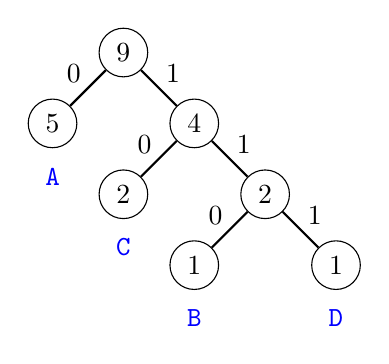
\begin{tikzpicture}[scale=0.9]
\node[draw, circle] (1) at (2,2) {$5$};
\node[draw, circle] (3) at (3,1) {$2$};
\node[draw, circle] (2) at (4,0) {$1$};
\node[draw, circle] (4) at (6,0) {$1$};
\node[draw, circle] (5) at (5,1) {$2$};
\node[draw, circle] (6) at (4,2) {$4$};
\node[draw, circle] (7) at (3,3) {$9$};

\node[color=blue] at (2,2-0.75) {\texttt{A}};
\node[color=blue] at (3,1-0.75) {\texttt{C}};
\node[color=blue] at (4,-0.75) {\texttt{B}};
\node[color=blue] at (6,-0.75) {\texttt{D}};

\node at (4.3,0.7) {0};
\node at (5.7,0.7) {1};
\node at (3.3,1.7) {0};
\node at (4.7,1.7) {1};
\node at (2.3,2.7) {0};
\node at (3.7,2.7) {1};

\path[draw,thick,-] (2) -- (5);
\path[draw,thick,-] (4) -- (5);
\path[draw,thick,-] (3) -- (6);
\path[draw,thick,-] (5) -- (6);
\path[draw,thick,-] (1) -- (7);
\path[draw,thick,-] (6) -- (7);
\end{tikzpicture}
\end{center}

Ara tots els nodes estan connectats en un arbre, i
podem recuperar la codificació llegint l'arbre:
\begin{center}
\begin{tabular}{rr}
caràcter & codi \\
\hline
\texttt{A} & 0 \\
\texttt{B} & 110 \\
\texttt{C} & 10 \\
\texttt{D} & 111 \\
\end{tabular}
\end{center}

\footnote{(N. del T.) Donem una intuïció de perquè la codificació de
Huffman és òptima.
Primer, en tota solució òptima passa que com més freqüent és un
caràcter, més curt és el seu codi. Altrament, intercanviaríem els codis
de dos caràcters que no complissin aquesta propietat i obtindríem una
codificació millor.
Per tant, els dos caràcters menys freqüents són els que tenen codis més llargs.
Aquests dos codis tenen la mateixa mida. Altrament, eliminaríem l'últim bit
del codi més llarg i obtindríem una codificació millor. Això és vàlid perquè el
nou codi escurçat no és part de la codificació perquè era un prefix, i no és
prefix de cap altre codi perquè els dos codis originals eren els més llargs. L'algorisme greedy descrit sorgeix d'aplicar repetidament aquesta propietat, i de fer servir l'arbre resultant per a generar una codificació òptima.}
